
\documentclass[letterpaper,hide notes,xcolor={table,svgnames},pdftex]{beamer}
\def\showexamples{t}


%\usepackage[svgnames]{xcolor}

%% Demo talk
%\documentclass[letterpaper,notes=show]{beamer}

\usecolortheme{crane}
\setbeamertemplate{navigation symbols}{}

\usetheme{MyPittsburgh}
%\usetheme{Frankfurt}

%\usepackage{tipa}

\usepackage{hyperref}
\usepackage{graphicx,xspace}
\usepackage[normalem]{ulem}

\newcommand\SF[1]{$\bigstar$\footnote{SF: #1}}



\newcounter{tmpnumSlide}
\newcounter{tmpnumNote}

% old question code
%\newcommand\question[1]{{$\bigstar$ \small \onlySlide{2}{#1}}}
% \newcommand\nquestion[1]{\ifdefined \presentationonly \textcircled{?} \fi \note{\par{\Large \textbf{?}} #1}}
% \newcommand\nanswer[1]{\note{\par{\Large \textbf{A}} #1}}


 \newcommand\mnote[1]{%
   \addtocounter{tmpnumSlide}{1}
   \ifdefined\showcues {~\tiny\fbox{\arabic{tmpnumSlide}}}\fi
   \note{\setlength{\parskip}{1ex}\addtocounter{tmpnumNote}{1}\textbf{\Large \arabic{tmpnumNote}:} {#1\par}}}

\newcommand\mmnote[1]{\note{\setlength{\parskip}{1ex}#1\par}}

%\newcommand\mnote[2][]{\ifdefined\handoutwithnotes {~\tiny\fbox{#1}}\fi
% \note{\setlength{\parskip}{1ex}\textbf{\Large #1:} #2\par}}

%\newcommand\mnote[2][]{{\tiny\fbox{#1}} \note{\setlength{\parskip}{1ex}\textbf{\Large #1:} #2\par}}

\newcommand\mquestion[2]{{~\color{red}\fbox{?}}\note{\setlength{\parskip}{1ex}\par{\Large \textbf{?}} #1} \note{\setlength{\parskip}{1ex}\par{\Large \textbf{A}} #2\par}\ifdefined \presentationonly \pause \fi}

\newcommand\blackboard[1]{%
\ifdefined   \showblackboard
  {#1}
  \else {\begin{center} \fbox{\colorbox{blue!30}{%
         \begin{minipage}{.95\linewidth}%
           \hspace{\stretch{1}} Some space intentionally left blank; done at the blackboard.%
         \end{minipage}}}\end{center}}%
         \fi%
}



%\newcommand\q{\tikz \node[thick,color=black,shape=circle]{?};}
%\newcommand\q{\ifdefined \presentationonly \textcircled{?} \fi}

\usepackage{listings}
\lstset{%
  keywordstyle=\bfseries,
  aboveskip=15pt,
  belowskip=15pt,
  captionpos=b,
  identifierstyle=\ttfamily,
  escapeinside={(*@}{@*)},
  stringstyle=\ttfamiliy,
  frame=lines,
  numbers=left, basicstyle=\scriptsize, numberstyle=\tiny, stepnumber=0, numbersep=2pt}

\usepackage{siunitx}
\newcommand\sius[1]{\num[group-separator = {,}]{#1}\si{\micro\second}}
\newcommand\sims[1]{\num[group-separator = {,}]{#1}\si{\milli\second}}
\newcommand\sins[1]{\num[group-separator = {,}]{#1}\si{\nano\second}}
\sisetup{group-separator = {,}, group-digits = true}

%% -------------------- tikz --------------------
\usepackage{tikz}
\usetikzlibrary{positioning}
\usetikzlibrary{arrows,backgrounds,automata,decorations.shapes,decorations.pathmorphing,decorations.markings,decorations.text}

\tikzstyle{place}=[circle,draw=blue!50,fill=blue!20,thick, inner sep=0pt,minimum size=6mm]
\tikzstyle{transition}=[rectangle,draw=black!50,fill=black!20,thick, inner sep=0pt,minimum size=4mm]

\tikzstyle{block}=[rectangle,draw=black, thick, inner sep=5pt]
\tikzstyle{bullet}=[circle,draw=black, fill=black, thin, inner sep=2pt]

\tikzstyle{pre}=[<-,shorten <=1pt,>=stealth',semithick]
\tikzstyle{post}=[->,shorten >=1pt,>=stealth',semithick]
\tikzstyle{bi}=[<->,shorten >=1pt,shorten <=1pt, >=stealth',semithick]

\tikzstyle{mut}=[-,>=stealth',semithick]

\tikzstyle{treereset}=[dashed,->, shorten >=1pt,>=stealth',thin]

\usepackage{ifmtarg}
\usepackage{xifthen}
\makeatletter
% new counter to now which frame it is within the sequence
\newcounter{multiframecounter}
% initialize buffer for previously used frame title
\gdef\lastframetitle{\textit{undefined}}
% new environment for a multi-frame
\newenvironment{multiframe}[1][]{%
\ifthenelse{\isempty{#1}}{%
% if no frame title was set via optional parameter,
% only increase sequence counter by 1
\addtocounter{multiframecounter}{1}%
}{%
% new frame title has been provided, thus
% reset sequence counter to 1 and buffer frame title for later use
\setcounter{multiframecounter}{1}%
\gdef\lastframetitle{#1}%
}%
% start conventional frame environment and
% automatically set frame title followed by sequence counter
\begin{frame}%
\frametitle{\lastframetitle~{\normalfont(\arabic{multiframecounter})}}%
}{%
\end{frame}%
}
\makeatother

\makeatletter
\newdimen\tu@tmpa%
\newdimen\ydiffl%
\newdimen\xdiffl%
\newcommand\ydiff[2]{%
    \coordinate (tmpnamea) at (#1);%
    \coordinate (tmpnameb) at (#2);%
    \pgfextracty{\tu@tmpa}{\pgfpointanchor{tmpnamea}{center}}%
    \pgfextracty{\ydiffl}{\pgfpointanchor{tmpnameb}{center}}%
    \advance\ydiffl by -\tu@tmpa%
}
\newcommand\xdiff[2]{%
    \coordinate (tmpnamea) at (#1);%
    \coordinate (tmpnameb) at (#2);%
    \pgfextractx{\tu@tmpa}{\pgfpointanchor{tmpnamea}{center}}%
    \pgfextractx{\xdiffl}{\pgfpointanchor{tmpnameb}{center}}%
    \advance\xdiffl by -\tu@tmpa%
}
\makeatother
\newcommand{\copyrightbox}[3][r]{%
\begin{tikzpicture}%
\node[inner sep=0pt,minimum size=2em](ciimage){#2};
\usefont{OT1}{phv}{n}{n}\fontsize{4}{4}\selectfont
\ydiff{ciimage.south}{ciimage.north}
\xdiff{ciimage.west}{ciimage.east}
\ifthenelse{\equal{#1}{r}}{%
\node[inner sep=0pt,right=1ex of ciimage.south east,anchor=north west,rotate=90]%
{\raggedleft\color{black!50}\parbox{\the\ydiffl}{\raggedright{}#3}};%
}{%
\ifthenelse{\equal{#1}{l}}{%
\node[inner sep=0pt,right=1ex of ciimage.south west,anchor=south west,rotate=90]%
{\raggedleft\color{black!50}\parbox{\the\ydiffl}{\raggedright{}#3}};%
}{%
\node[inner sep=0pt,below=1ex of ciimage.south west,anchor=north west]%
{\raggedleft\color{black!50}\parbox{\the\xdiffl}{\raggedright{}#3}};%
}
}
\end{tikzpicture}
}


%% --------------------

%\usepackage[excludeor]{everyhook}
%\PushPreHook{par}{\setbox0=\lastbox\llap{MUH}}\box0}

%\vspace*{\stretch{1}

%\setbox0=\lastbox \llap{\textbullet\enskip}\box0}

\setlength{\parskip}{\fill}

\newcommand\noskips{\setlength{\parskip}{1ex}}
\newcommand\doskips{\setlength{\parskip}{\fill}}

\newcommand\xx{\par\vspace*{\stretch{1}}\par}
\newcommand\xxs{\par\vspace*{2ex}\par}
\newcommand\tuple[1]{\langle #1 \rangle}
\newcommand\code[1]{{\sf \footnotesize #1}}
\newcommand\ex[1]{\uline{Example:} \ifdefined \presentationonly \pause \fi
  \ifdefined\showexamples#1\xspace\else{\uline{\hspace*{2cm}}}\fi}

\newcommand\ceil[1]{\lceil #1 \rceil}


\AtBeginSection[]
{
   \begin{frame}
       \frametitle{Outline}
       \tableofcontents[currentsection]
   \end{frame}
}



\pgfdeclarelayer{edgelayer}
\pgfdeclarelayer{nodelayer}
\pgfsetlayers{edgelayer,nodelayer,main}

\tikzstyle{none}=[inner sep=0pt]
\tikzstyle{rn}=[circle,fill=Red,draw=Black,line width=0.8 pt]
\tikzstyle{gn}=[circle,fill=Lime,draw=Black,line width=0.8 pt]
\tikzstyle{yn}=[circle,fill=Yellow,draw=Black,line width=0.8 pt]
\tikzstyle{empty}=[circle,fill=White,draw=Black]
\tikzstyle{bw} = [rectangle, draw, fill=blue!20, 
    text width=4em, text centered, rounded corners, minimum height=2em]
    
    \newcommand{\CcNote}[1]{% longname
	This work is licensed under the \textit{Creative Commons #1 3.0 License}.%
}
\newcommand{\CcImageBy}[1]{%
	\includegraphics[scale=#1]{creative_commons/cc_by_30.pdf}%
}
\newcommand{\CcImageSa}[1]{%
	\includegraphics[scale=#1]{creative_commons/cc_sa_30.pdf}%
}
\newcommand{\CcImageNc}[1]{%
	\includegraphics[scale=#1]{creative_commons/cc_nc_30.pdf}%
}
\newcommand{\CcGroupBySa}[2]{% zoom, gap
	\CcImageBy{#1}\hspace*{#2}\CcImageNc{#1}\hspace*{#2}\CcImageSa{#1}%
}
\newcommand{\CcLongnameByNcSa}{Attribution-NonCommercial-ShareAlike}

\newenvironment{changemargin}[1]{% 
  \begin{list}{}{% 
    \setlength{\topsep}{0pt}% 
    \setlength{\leftmargin}{#1}% 
    \setlength{\rightmargin}{1em}
    \setlength{\listparindent}{\parindent}% 
    \setlength{\itemindent}{\parindent}% 
    \setlength{\parsep}{\parskip}% 
  }% 
  \item[]}{\end{list}} 




\usepackage{alltt}

\title{Lecture 5 --- XML, Android, IDEs}

\author{Patrick Lam \& Jeff Zarnett \\ \small \texttt{p.lam@ece.uwaterloo.ca} \& \texttt{jzarnett@uwaterloo.ca}}
\institute{Department of Electrical and Computer Engineering \\[-1ex]
  University of Waterloo}
\date{\today}


\begin{document}


\begin{frame}
  \titlepage

\end{frame}

\part{XML}
\frame{\partpage}

\begin{frame}
\frametitle{eXtensible Markup Language}
\begin{changemargin}{1cm}
You need to know a bit about
XML (e\textbf{X}tensible \textbf{M}arkup \textbf{L}anguage)  to build Android applications 

By
the way, this is examinable material.

For further reading, you can consult many resources on the Web.
Here's one:
\begin{center}
\url{http://www.w3schools.com/xml/default.asp}
\end{center}

\end{changemargin}
\end{frame}

\begin{frame}
\frametitle{XML in one Line}
\begin{changemargin}{1cm}
\begin{center}
{\Large XML is a \emph{structured document format}.}
\end{center}
\end{changemargin}
\end{frame}

\begin{frame}
\frametitle{Structured Document Format}
\begin{changemargin}{1cm}
All XML documents therefore have the same format. 

XML has no intrinsic meaning. 

It just separates content from structure. 

It is meant to be human-readable/writable.

If you are familiar with HTML, there are a number of similarities, but XML is more general. 

\end{changemargin}
\end{frame}

\begin{frame}[fragile]
\frametitle{XML Document Terminology}
\begin{changemargin}{1cm}

Every XML document begins with \verb+<?xml version="1.0" encoding="utf-8"?>+

Documents have \alert{tags}, which appear between angle brackets:\\
\quad \texttt{<example>}

Tags are opened and closed, so that tag must be followed by \texttt{</example>}, which closes the \texttt{example} tag. 

We can also have ``self-closing'' tabs, (notational convenience) such as \texttt{<approval/>}.

A tag may also have attributes, like colour in this example: \texttt{<square colour=``red''/>}.

\end{changemargin}
\end{frame}

\begin{frame}
\frametitle{XML Parsing}
\begin{changemargin}{1cm}

XML is intended to be human-readable and human writeable. 

Computers can read and comprehend XML by ``parsing'' the document. 

There are a number of well-known XML parsers.

Use one of them if you need to programmatically examine some XML and do not write your own.

\end{changemargin}
\end{frame}


\begin{frame}[fragile]
\frametitle{Android Manifest}
\begin{changemargin}{1cm}
Example XML Document: Android Manifest.


(Shown from the notes because it's too large for slides).

\end{changemargin}
\end{frame}


\begin{frame}[fragile]
\frametitle{XML Tree Structure}
\begin{changemargin}{1cm}

XML is tree-structured: at the top level, there is a \emph{root} element. We can convert the textual form into a tree.

\begin{center}
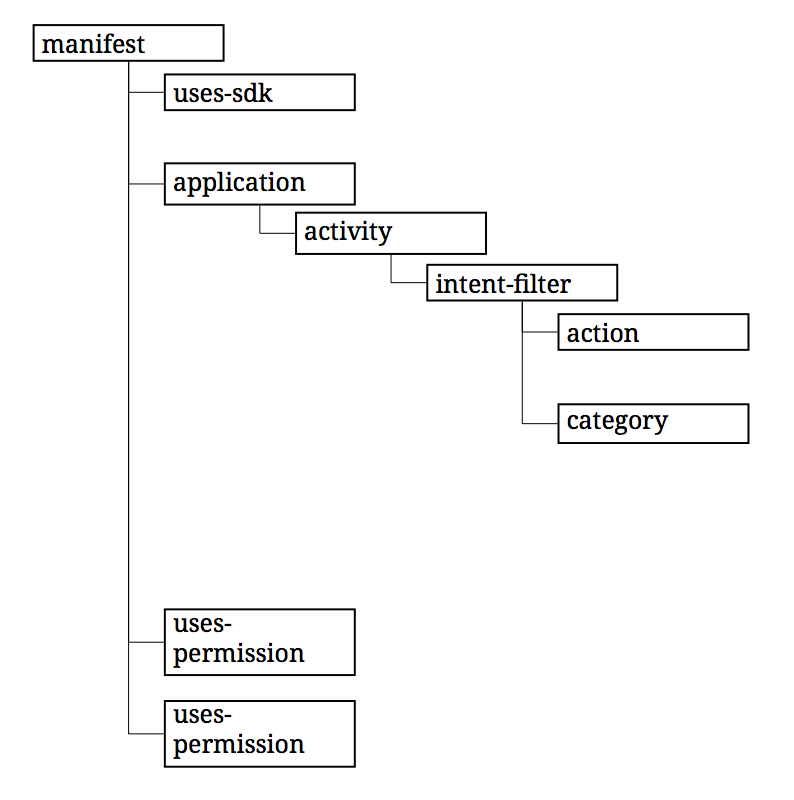
\includegraphics[width=0.5\textwidth]{images/XML-Structure.png}
\end{center}

\end{changemargin}
\end{frame}

\part{Android Programming}
\frame{\partpage}

\begin{frame}
\frametitle{Android: Introduction}
\begin{changemargin}{1cm}

By now you have no doubt taken a look at the labs.

You need to implement them using Android, either on your own phone or one of the devices we provide in the labs. 

We will take some time to introduce you to Android programming.

\end{changemargin}
\end{frame}


\begin{frame}
\frametitle{Android: Activity}
\begin{changemargin}{1cm}

``An activity is a single, focused thing that the user can do.''

Usually, an Activity corresponds to a full-screen window which 
the user may interact with. For instance, the user may:
\begin{itemize}
\item set up a timer; 
\item read off sensor values; or
\item make a phone call.
\end{itemize}

\end{changemargin}
\end{frame}

\begin{frame}
\frametitle{Android: Activity}
\begin{changemargin}{1cm}

Applications may contain multiple activities, each of which
corresponds to a thing that the user wants to do.  

Android organizes
activities into tasks.  

A task consists of a last-in, first-out stack
of activities, possibly from different applications.

\end{changemargin}
\end{frame}


\begin{frame}
\frametitle{The Back Button}
\begin{changemargin}{1cm}

The Back button pops the topmost activity off the stack and gets rid of it.

\begin{center}
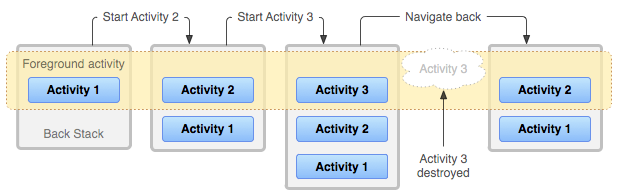
\includegraphics[width=0.9\textwidth]{images/diagram_backstack.png}
\end{center}

\end{changemargin}
\end{frame}

\begin{frame}
\frametitle{Multitasking}
\begin{changemargin}{1cm}

It is also possible to switch between tasks.

Switching tasks puts a different activity and its stack
in the foreground, and puts the old activity in the background.

\begin{center}
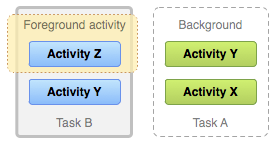
\includegraphics[width=0.7\textwidth]{images/diagram_multitasking}
\end{center}

\end{changemargin}
\end{frame}


\begin{frame}
\frametitle{Doing Something in the Activity}
\begin{changemargin}{1cm}

You'll be writing a lot of code in \texttt{onCreate()}. 

It gets executed when the activity 
starts. 

Typically, it will set up the user interface, namely:
\begin{itemize}
\item creating widgets;
\item setting up event listeners;
\end{itemize}

Note that you must call {\texttt{\textbf{super.onCreate()}}}. \\
\quad This is done for you in the autogenerated boilerplate code.


\end{changemargin}
\end{frame}

\begin{frame}
\frametitle{Retrieving Widgets}
\begin{changemargin}{1cm}

If you've declared widgets in the
XML file, you can use the {\texttt{\textbf{findViewById()}}} method
to get a hold of them. 

Note:
\begin{itemize}
\item you need to cast the return value, e.g. \\
\texttt{\textbf{tv = (TextView) findViewById(R.id.t);}}
\item you must save the XML file to get the right ids on the {\tt R} object.
\end{itemize}

\end{changemargin}
\end{frame}

\begin{frame}
\frametitle{Programmatically Adding Widgets}
\begin{changemargin}{1cm}

We ask you to
add widgets programmatically in Lab 1. There are two steps:
\begin{enumerate}
\item Create the widget: 
\texttt{\textbf{~tv = new TextView(getApplicationContext());}} 
\item Add it to the Activity:
\texttt{\textbf{~addView(tv);}}
\end{enumerate}
\end{changemargin}
\end{frame}

\begin{frame}
\frametitle{Activity Lifecycle}
\begin{changemargin}{1cm}

Although we've only talked about {\tt onCreate()}, there are numerous
other methods on {\tt Activity} which Android calls at various times.

\begin{center}
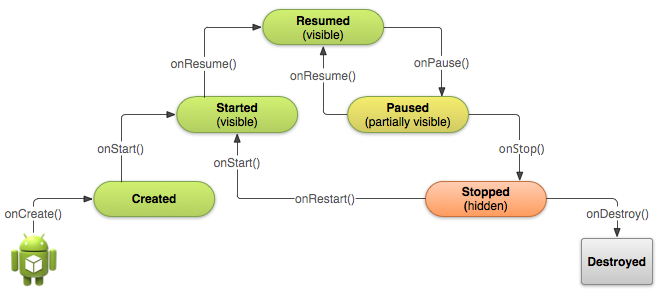
\includegraphics[width=.9\textwidth]{images/basic-lifecycle}
\end{center}


\end{changemargin}
\end{frame}


\part{Integrated Development Environments}
\frame{\partpage}

\begin{frame}
\frametitle{In the Dark Ages}
\begin{changemargin}{1cm}

Write code in editor (\texttt{vi}, \texttt{emacs}, \texttt{notepad.exe})

Invoke command-line compiler

Can we make better tools? Yes: IDE! \mnote{The IDE concept has been around for over 25 years.}

\end{changemargin}
\end{frame}


\begin{frame}
\frametitle{What is an IDE?}

\begin{changemargin}{1cm}
\Large
Contains:
\begin{itemize}
\item editor, plus
\item compiler, plus
\item debugger
\end{itemize}

Integrated into a single environment.

\end{changemargin}

\end{frame}

\begin{frame}
\frametitle{The Eclipse IDE}

\begin{changemargin}{1cm}
\large
Eclipse is a fully-featured modern IDE.\\[1em]

Notes:
\begin{itemize}
\item runs on Linux, Mac, Windows;
\item it is free software: you can extend and modify it;
\item initially developed by IBM Ottawa.
\end{itemize}

\mnote{By now you have worked with Eclipse in the labs and presumably you used Microsoft Visual Studio when programming in C\# for ECE~150.}

\end{changemargin}
\end{frame}

\begin{frame}
\frametitle{Beyond Core IDE Components}

\begin{changemargin}{1cm}
\large
Eclipse (and other IDEs) also support:

\begin{itemize}
\item revision control systems (you've used this); 
\item documentation and modelling (e.g. UML);
\item autocomplete and refactoring.
\end{itemize}

\end{changemargin}
\end{frame}

\begin{frame}
\frametitle{Syntax Highlighting}
\begin{changemargin}{1cm}

\begin{center}
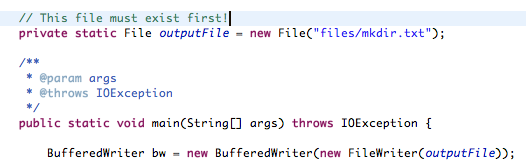
\includegraphics[width=0.75\textwidth]{images/highlight.png}
\end{center}

\mnote{The IDE highlights different syntax of the program, by making them different colours. It makes it easier to see and understand different parts of the code, and makes it possible to detect errors.} 

\end{changemargin}
\end{frame}


\begin{frame}
\frametitle{Syntax Highlighting}
\begin{changemargin}{1cm}

\begin{center}
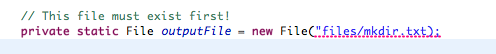
\includegraphics[width=0.75\textwidth]{images/highlight2.png}
\end{center}


\mnote{For example, if you forgot a '' (close-quote) character at the end of a string, then subsequent code after where you expect will be string-coloured, revealing the error. Similarly, comments are often coloured so you can see at a glance if half a line is commented out.}


\end{changemargin}
\end{frame}

\begin{frame}
\frametitle{Templates}
\begin{changemargin}{1cm}

IDEs often allow you to start your
project from a template; easier than starting from scratch

\begin{itemize}
\item Android Test Project (you'll use these);
\item Java Project
\item Java Class
\item Java Interface
\end{itemize}

\end{changemargin}
\end{frame}

\begin{frame}
\frametitle{Continuous Compiling}
\begin{changemargin}{1cm}

\begin{center}
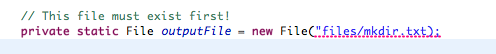
\includegraphics[width=0.75\textwidth]{images/highlight2.png}
\end{center}

Notice the red squiggle under the error.\mnote{ Instead of manually invoking the compiler manually, modern IDEs are constantly running the compiler when a file is changed. So as you're working, you'll see errors and warnings right away.

When you get a red (or yellow) squiggle underneath your code (see the figure below) there's an error (or warning). Eclipse and other very clever IDEs can sometimes suggest a solution, in a feature known as quick fix}

\end{changemargin}
\end{frame}



\begin{frame}
\frametitle{Project Development Workflow}

\begin{changemargin}{1cm}
\Large
\begin{enumerate}
\setcounter{enumi}{-1}
\item Figure out what you'll need to do.
\item Start a new project from a template or, more realistically,
  check it out from a version control repository.
\item Make the edits that you need. 
\item Test your edits by running the application.
\item Debug your edits.
\item Commit your files to the version control repository.
\end{enumerate}
\end{changemargin}
\end{frame}

\begin{frame}
\frametitle{Eclipse demo}

\begin{changemargin}{1cm}
We'll show a little demo of Eclipse (time permitting):
\begin{enumerate}
	\item Create a new Android project from a \structure{template}.
	\item Go over syntax highlighting.
	\item Show you content assist.
	\item Demonstrate the ``Quick Fix'' feature.
\end{enumerate}
\end{changemargin}

\end{frame}


\end{document}

